\newcommand{\formula}[1]{\mathit{formula}(#1)}
\newcommand{\probability}[1]{\mathit{prob}(#1)}

\section{Monitoring Probabilistic Constraints}
\label{sec:monitoring}
In Section~\ref{sec:scenarios}, we have shown how we can take a \pdeclare model and generate its constraint scenarios, together with their corresponding probability intervals. We now describe how this technique can be directly turned into an operational probabilistic monitoring and conformance checking framework.

Let $M = \tup{\Sigma,\mathcal{C}}$ be a \pdeclare model with $n$ probabilistic constraints. For simplicity, we do not distinguish between crisp and genuinely probabilistic constraints, nor prune away implausible scenarios: the produced monitoring results do not change, but obviously our implementation, presented at the end of this section, takes into account these aspects for optimization reasons.
%
$M$ generates $2^n$ constraint scenarios. As discussed in Section~\ref{sec:scenarios}, each scenario $S$ comes with a corresponding characteristic \LTLf formula, which amounts to the conjunction of positive and negated constraints in $\mathcal{C}$, where the decision of which ones are taken positive and which negative is defined by the scenario itself. We denote such a formula by $\formula{S}$. For example, if $\mathcal{C} = \set{\tup{\varphi_1,p_1},\tup{\varphi_2,p_2},\tup{\varphi_3,p_3}}$,  then $\formula{S_{101}}=\varphi_1 \land \neg \varphi_2 \land \varphi_3$.
%
In addition, each scenario $S$ comes with its probability interval, calculated by minimizing and maximizing its probability variable in the system of inequalities $\Lmc_M$. We denote such a probability interval by $\probability{S}$. From Example \ref{ex:intervals}, we have, e.g., that $\probability{S_{10}}= [0.7,0.8]$.

Since the characteristic formula of a scenario is in standard $\LTLf$, we can construct a \emph{scenario monitor} by recasting well-known techniques \cite{MMWV11,DDGM14}. Specifically, given an $\LTLf$ formula $\varphi$ over a set $\Sigma$ of activities, and a partial trace $\tau$ representing an ongoing process execution, a monitor outputs one of the four following truth values:
\begin{compactitem}[$\bullet$]
\item $\tau$ \emph{(permanently) satisfies} $\varphi$, if $\varphi$ is currently satisfied ($\tau \models \varphi$), and $\varphi$ stays satisfied no matter how the execution continues, that is, for every possible continuation trace $\tau'$ over $\Sigma$, we have $\tau \cdot \tau' \models \varphi$ (the $\cdot$ operator denotes the concatenation of two traces);
\item $\tau$ \emph{possibly satisfies} $\varphi$, if $\varphi$ is currently satisfied ($\tau \models \varphi$), but $\varphi$ may become violated in the future, that is, there exists a continuation trace $\tau'$ over $\Sigma$ such that $\tau \cdot \tau' \not\models \varphi$;
\item $\tau$ \emph{possibly violates} $\varphi$, if $\varphi$ is currently violated ($\tau \not\models \varphi$), but $\varphi$ may become satisfied in the future, that is, there exists a continuation trace $\tau'$ over $\Sigma$ such that $\tau \cdot \tau' \models \varphi$;
\item $\tau$ \emph{(permanently) violates} $\varphi$, if $\varphi$ is currently violated ($\tau \not\models \varphi$), and $\varphi$ stays violated no matter how the execution continues, that is, for every possible continuation trace $\tau'$ over $\Sigma$, we have $\tau \cdot \tau' \not\models \varphi$.
\end{compactitem}
In \cite{MMWV11,DDGM14}, it is shown that a monitor producing such outputs can be seamlessly obtained by constructing and determinizing the finite-state automaton $\aut_\varphi$ for $\varphi$, and assigning each automaton state to one of the four truth values.

%\input{monitor}
\begin{figure*}[t!]
	\centering	
		\begin{tabular}{ c  c  }
			\makecell{			
				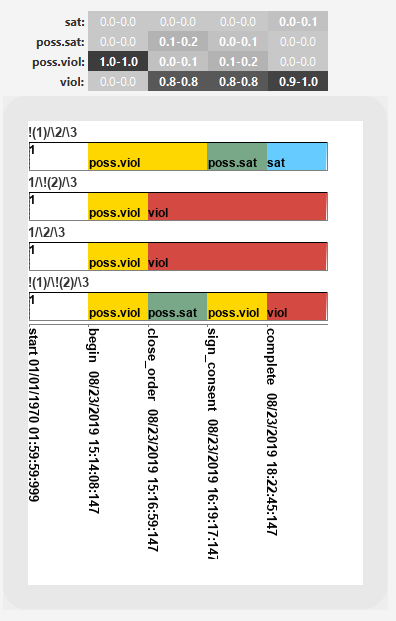
\includegraphics[width=0.5\textwidth]{images/LTL2Automaton_01_log_c_r.png}			
			}
			&
			\makecell{		
				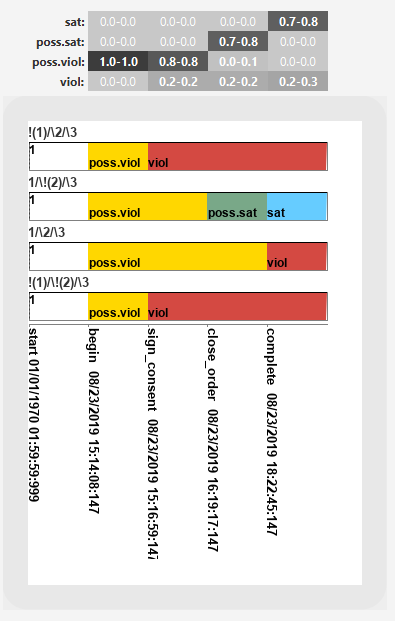
\includegraphics[width=0.5\textwidth]{images/LTL2Automaton_01_log_r_c.png}			
			} \\
			 trace $\tup{\activity{close},\activity{sign}}$ & trace $\tup{\activity{sign},\activity{close}}$
		\end{tabular}
	\caption{Output of the implemented tool on the example in \figurename\ref{fig:scenarios-2}.}
	\label{fig:ex0t1}
\end{figure*}

We proceed as follows. For each plausible constraint scenario $S$ over $M$, we construct the finite-state automaton $\aut_{\formula{S}}$, and turn it into a monitor as described above.\footnote{Implausible scenarios are irrelevant, since they produce an output that is associated to probability $0$, and would be therefore discarded when computing the aggregated probability intervals.} We then track the evolution of a running trace by delivering its events to \emph{all} such monitors in parallel, returning the truth values they produce. Note that, at runtime, we do not know in which scenario the trace will fall when completed. Hence, we actually do not know the exact truth value of the trace. For this reason, we compute the truth value of the trace probabilistically by aggregating the probabilities of the scenarios that produce the same truth value. In particular, we compute the \emph{aggregated probability interval} for each truth value, by taking the system of inequalities $\Lmc_M$ and calculating the extreme values of the aggregated interval by minimizing/maximizing the sum of the probability variables associated to the scenarios that produce that truth value. The aggregated probabilities give an indication of how probable it is that the trace can be associated to each specific truth value.

When a trace ends (which is signalled by a special, \emph{complete} event) all monitors currently outputting \emph{possible satisfaction} turn to \emph{permanent satisfaction}, and those outputting \emph{possible violation} turn to \emph{permanent violation}. Hence, when a trace ends, it either permanently violates all scenarios (thus being classified as a non-conforming one), or permanently violates all scenarios but one, which is permanently satisfied and consequently witnesses that the trace belongs to that scenario. Notably, this can be instrumental to classify traces into process variants.

%Interestingly, all monitors may agree on violation outputs, witnessing the non-conformance of the monitored trace. If, instead, monitors produce different outputs, their corresponding aggregated probabilities give a probabilistic indication of conformance that depends on how likely it is for the monitored trace to belong to the different plausible scenarios. The more the trace evolves, the more it becomes clear to which scenario it belongs, and in turn whether it configures itself as a common trace (belonging to a highly plausible scenario) or as an outlier one (belonging to a less plausible scenario).


\begin{example}
  Consider the \pdeclare model in Figure~\ref{fig:scenarios} with its three plausible scenarios (recall that four scenarios are logically plausible there, but one of those has probability $0$, so only three remains to be monitored). Figure~\ref{fig:monitoring} shows the result produced when monitoring a trace that at some point appears to belong to the most plausible scenario, but in the end turns out to conform to the less plausible one. From the image, we can also clearly see that the trace consisting only of a close order activity would be judged as non-conforming, as it would violate all scenarios.
\end{example}

This probabilistic monitoring technique has been fully implemented.\footnote{\url{https://bitbucket.org/fmmaggi/probabilisticmonitor/src/master/}} For solving systems of inequalities, we use the Java based LP solver\footnote{\url{http://lpsolve.sourceforge.net/5.5/}}. The implementation comes with various optimizations. First, scenarios are computed by directly imposing that crisp constraints with probability $1$ must hold in their positive form in all scenarios. Second, only plausible scenarios are retained for monitoring. Third, the results obtained by minimizing and maximizing for aggregate probability variables are cached, to avoid solving multiple times the same problem.
\figurename \ref{fig:ex0t1} shows the output of the implemented monitoring tool on the example in \figurename \ref{fig:scenarios-2} and for two different traces.\footnote{In the screenshots, 1 and 2 represent the probabilistic constraints labeled with 1 and 2 in \figurename \ref{fig:scenarios-2}, whereas 3 represents the crisp constraint in the same example.} Here, the aggregated probability intervals are shown with a dark gray or light gray background depending on whether their midpoint is closer to 1 or to 0, respectively, thus giving an indication of the most probable truth values for the monitored trace. The first trace (on the left) is classified as belonging to scenario $S_{01}$ and is an outlier because this scenario has low probability (corresponding to a probability interval of $\probability{S_{01}}= [0.0,0.1]$). The second trace (on the right) is classified as belonging to the highly plausible scenario $S_{10}$ (corresponding to a probability interval of $\probability{S_{10}}= [0.7,0.8]$).





